\documentclass[aspectratio=169,
				xcolor=table]{beamer}

% Load general definitions
\usepackage[utf8]{inputenc}
%\usepackage[T1]{fontenc}
\usepackage[brazil]{babel}
\usepackage{amsmath}
\usepackage{amsfonts}
\usepackage{amssymb}
\usepackage{graphicx}
\usepackage{verbatim}
\usepackage{cancel}
\usepackage{askmaps}
\usepackage{tabularx}
\usepackage[table]{xcolor}
%\usepackage{tikz}
\usepackage{multirow}
\usepackage{mathtools}
\usepackage{color, colortbl}
\usepackage{etoolbox}
\usepackage{pbox}
\usepackage{changepage}
\usepackage{xpatch}
\usepackage{array}
\usepackage{marvosym}
\usepackage{tabu}
\usepackage{multicol}
\usepackage{listings}
\usepackage{underscore}
\usepackage{filecontents}
\usepackage[]{algorithm2e}
\usepackage{ragged2e}

\newcolumntype{P}[1]{>{\centering\arraybackslash}m{#1}}
\definecolor{Gray}{gray}{0.75}
\definecolor{Gray2}{gray}{0.85}

\definecolor{lightBlue}{HTML}{DAE8FC}
\definecolor{Blue}{RGB}{51, 51, 204}

%\useinnertheme[lily]{rounded}
\usetheme{UniEvangelica}
%\usetheme{Copenhagen}
%\usetheme{Berlin}
%\usecolortheme{dolphin}
\tolerance=1
\emergencystretch=\maxdimen
\hyphenpenalty=10000
\hbadness=10000

\setbeamertemplate{navigation symbols}{}%remove navigation symbols


\let\olditem=\item% 
\renewcommand{\item}{\olditem \justifying}%
\def\center{\trivlist \centering\item\relax}
\def\endcenter{\endtrivlist}

\setbeamertemplate{itemize/enumerate body begin}{\large}
\setbeamertemplate{itemize/enumerate subbody begin}{\large}

\setbeamertemplate{itemize item}{\raisebox{0.1ex}{$\blacktriangleright$}\hskip0.1em}
\setbeamertemplate{itemize subitem}{\raisebox{0.1ex}{$\blacktriangleright$}\hskip0.1em}

\newcommand{\greenarrow}{\textcolor{green}{\rotatebox[origin=c]{180}{\MVArrowDown}}}

\newcommand{\redarrow}{\textcolor{red}{\MVArrowDown}}

%\newcommand{\ftable}{
%	\begin{table}
%		\large
%		\centering
%		\rowcolors{1}{\ifnumless{\rownum}{2}{Blue}{lightBlue}}{}
%}

\newenvironment{eftable}{
	\begin{table}
		\large
		\centering
		\rowcolors{1}{}{Blue}
		\rowcolors{1}{\ifnumless{\rownum}{2}{Blue}{lightBlue}}{}
	}
	{
	\end{table}
}


%\setbeamertemplate{frametitle}
%{
%	%\vspace*{-2em}	
%	\insertframetitle
%
%	 %\textcolor{white}{\LARGE \insertframetitle}
%
%}

% Specific definitions
\institute[]{\uppercase{Engenharia da Computação}}
\title[]{Prática em Fábrica de Software III}
\subtitle[]{\uppercase{Controladores Lógico Programáveis}}
\author[]{Prof. Alexandre Tannus}
\date{}
\AtBeginSection{\frame{\tableofcontents[currentsection]}}

\begin{document}
	\begin{frame}
		\titlepage
	\end{frame}
	
	\begin{frame}{Questionamentos}
		\begin{itemize}
			\item O que é automação?
			\vspace{1em}
			\item Existe diferença entre mecanização e automação?
			\vspace{1em}
			\item Onde pode ser aplicada a automação?
			\vspace{1em}
			\item Por que automatizar?
		\end{itemize}		
	\end{frame}
	
	\begin{frame}{Definição}
		\begin{itemize}
			\item Automação
			\begin{itemize}
				\item Sistema de equipamentos eletrônicos e/ou mecânicos que controlam seu próprio funcionamento
				\item "Qualquer sistema, apoiado em computadores, que substitui o trabalho humano, em favor da segurança das pessoas, da qualidade dos produtos, rapidez da produção ou da redução de custos, assim aperfeiçoando os complexos objetivos das indústrias, dos serviços ou bem estar” (Moraes e Castrucci, 2007)
			\end{itemize}
			\vspace{0.7em}
			\item Mecanização
			\begin{itemize}
				\item Uso de máquinas para realizar um trabalho, substituindo assim o esforço físico do homem
			\end{itemize}
		\end{itemize}
	\end{frame}
	
	\begin{frame}{Evolução da automação}
		\begin{figure}[hbtp]
		\centering
		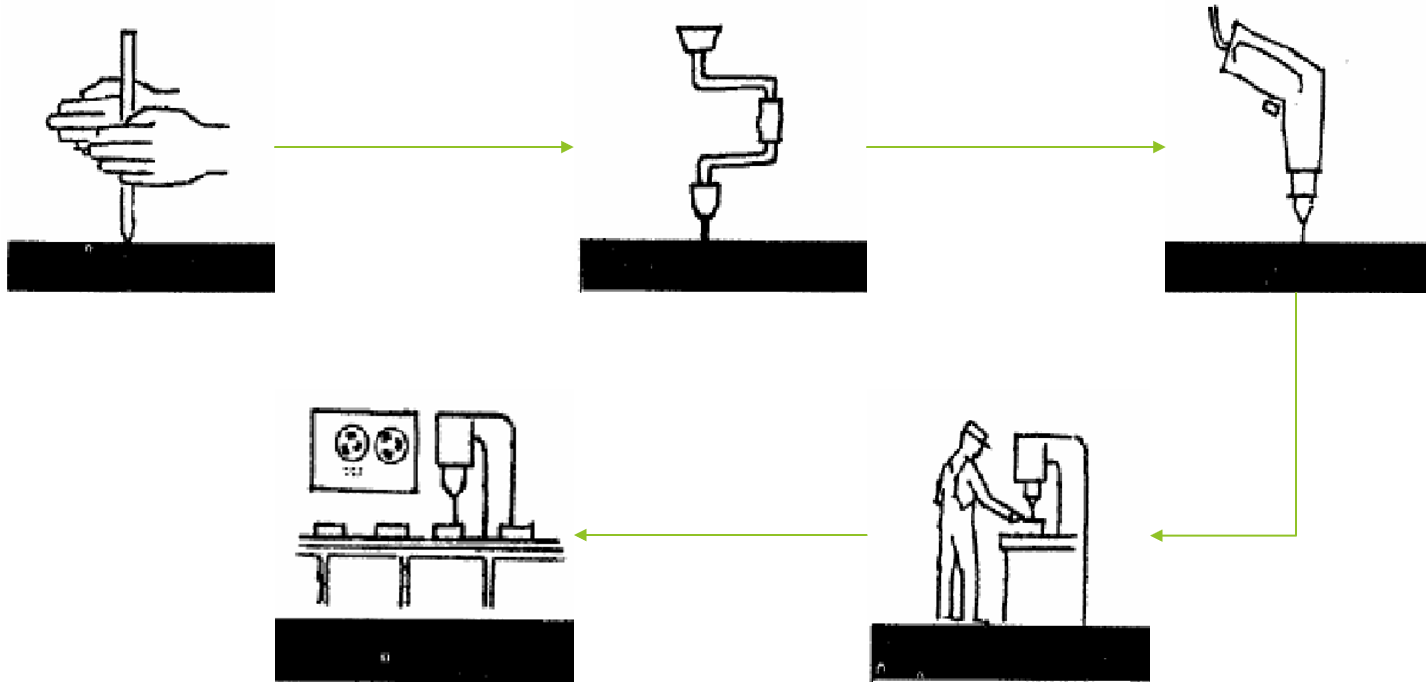
\includegraphics[height=5cm, keepaspectratio]{../figs/cap04/automacao.png}
		\end{figure}		
	\end{frame}
	
	\begin{frame}{Histórico}
		\begin{itemize}
			\item Mecanização
			\begin{itemize}
				\item Invenção da roda
				\item Moinhos de vento
				\item Rodas d'água
			\end{itemize}
			\vspace{1em}
			\item Automação
			\begin{itemize}
				\item Revolução Industrial - século XVIII - James Watt
			\end{itemize}
		\end{itemize}
	\end{frame}
	
	\begin{frame}{Histórico}
		\begin{columns}
			\begin{column}{0.5\textwidth}
			
				\begin{itemize}
					\item 1870
					\begin{itemize}
						\item Energia elétrica na indústria
					\end{itemize}
					\vspace{1em}
					\item 1880
					\begin{itemize}
						\item Cartões perfurados - Hollerith
					\end{itemize}
				\end{itemize}
			\end{column}
			\begin{column}{0.5\textwidth}
				\begin{figure}[hbtp]
				\centering
				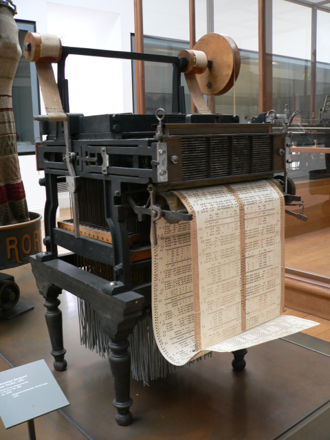
\includegraphics[height=5cm, keepaspectratio]{../figs/cap04/hollerith.png}
				\end{figure}			
			\end{column}
		\end{columns}
	\end{frame}
	\section{Histórico}
	\begin{frame}{Histórico}
	
		\begin{columns}
			\begin{column}{0.6\textwidth}
				\begin{itemize}
					\item 1946 - Primeira geração - Válvulas e relés
						\begin{itemize}
							\item ENIAC
							\item 180 $m^2$
							\item 30 toneladas
							\item 150 kW
							\item 5000 cálculos por segundo
						\end{itemize}			
					\vspace{1em}
					\item 1952 - Segunda geração - Transistores
				\end{itemize}
			\end{column}
			\begin{column}{0.4\textwidth}
				\begin{figure}[hbtp]
				\centering
				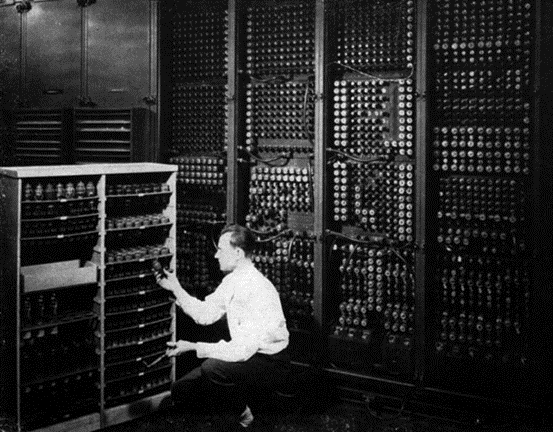
\includegraphics[width=.95\textwidth, keepaspectratio]{../figs/cap04/eniac.png}
				\end{figure}			

			\end{column}
		\end{columns}
	\end{frame}
	
	\begin{frame}{Histórico}
		\begin{columns}
			\begin{column}{0.6\textwidth}
				\begin{itemize}
					\item Terceira geração - Circuitos Integrados
					\begin{itemize}
						\item Milhares de transistores
						\item Pastilha de silício de 1 $cm^2$
						\item Aumento da capacidade de processamento
					\end{itemize}					
					\vspace{1em}
					\item 1975 - Quarta geração - VLSI
					\begin{itemize}
						\item Computadores pessoais
					\end{itemize}
				\end{itemize}
				
			\end{column}
			\begin{column}{0.4\textwidth}
				\begin{figure}[hbtp]
				\centering
				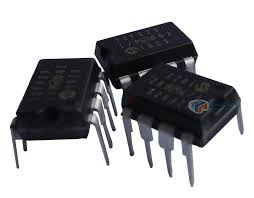
\includegraphics[height=2cm, keepaspectratio]{../figs/cap04/transistor.png}
				\end{figure}	
				
				\begin{figure}[hbtp]
				\centering
				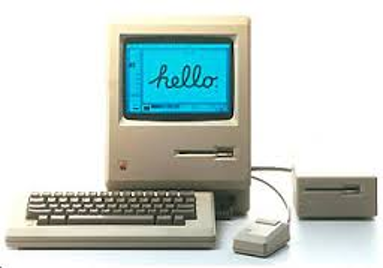
\includegraphics[width=.75\textwidth, keepaspectratio]{../figs/cap04/lisa.png}
				\end{figure}	
			\end{column}
		\end{columns}
	\end{frame}
	
	\begin{frame}{Controlador Lógico Programável - CLP}
		\begin{itemize}
			\item Richard Morley - 1968
			\vspace{1em}
			\item Especificação dos primeiros controladores
			\begin{itemize}
				\item Facilidade de programação
				\item Facilidade de manutenção 
				\item Alta confiabilidade
				\item Dimensões menores
				\item Envio de dados para processamento centralizado
				\item Expansão em módulos
				\item Preço competitivo

			\end{itemize}
		\end{itemize}
	\end{frame}
	
	\begin{frame}{Evolução dos CLPs}
		\begin{itemize}
			\item Primeira geração
			\begin{itemize}
				\item Transistores
				\item Circuitos integrados
				\item Baixa escala de integração
			\end{itemize}
			\vspace{1em}
			\item Década de 1970
			\begin{itemize}
				\item Maior poder de processamento
				\item Maior número de entradas e saídas
				\item Novas funções
				\item Diminuição de custos e tamanho
				\item Aumento do poder de processamento e confiabilidade
			\end{itemize}
		\end{itemize}
	\end{frame}
	
	\begin{frame}{Modelos}
		\begin{itemize}
			\item Modicon 084 - 1969
			\item Modicon 284
			\begin{itemize}
				\item 80 entradas
				\item 40 saídas
			\end{itemize}
			\item Modicon 1084
			\begin{itemize}
				\item 5120 entradas e saídas
			\end{itemize}
		\end{itemize}
	\end{frame}	
	
	\begin{frame}{Modelos}
	
		\begin{itemize}
			\item Micro 84 - 1977
			\begin{itemize}
				\item 64 entradas e saídas
				\item Temporizadores
				\item Contadores
				\item Sequenciadores
				\item Funções matemáticas
			\end{itemize}
			\vspace{1em}
			\item 984
			\begin{itemize}
				\item Funções PID
			\end{itemize}
		\end{itemize}
		
	\end{frame}
	
	\begin{frame}{Fabricantes}
		\begin{itemize}
			\item Modicon
			\vspace{1em}
			\item Allen Bradley
			\begin{itemize}
				\item PDQ – 1959
				\item PLC – 1970
				\item PLC 2 – 1975
				\item PLC 2/20 – 1979

			\end{itemize}
			\vspace{1em}
			\item Texas Instruments
			
		\end{itemize}
	\end{frame}
	\section{Caracteríticas Técnicas}
	\begin{frame}{Controladores Lógico Programáveis}
		\begin{itemize}
			\item Sequenciamento de funções 
			\vspace{1em}
			\item Controle realimentado
			\vspace{1em}
			\item Tipos de CLP
			\begin{itemize}
				\item Tipo 1 – Somente sequenciamento de funções
				\item Tipo 2 – Somente controle realimentado
				\item Tipo 3 – Ambas as funções
			\end{itemize}
		\end{itemize}
	\end{frame}
	
	\begin{frame}{Definição}
		\begin{block}{ABNT}
			O CLP é um equipamento eletrônico digital com  hardware e  software compatíveis com aplicações industriais.
		\end{block}

		\begin{block}{NEMA}
			Aparelho  eletrônico  digital  que  utiliza  uma  memória programável  para armazenamento  interno  de  instruções  para  implementações  específicas,  como  lógica, sequenciamento, temporização, contagem e aritmética, para controlar, através de módulos de entradas e saídas, vários tipos de máquinas ou processos

		\end{block}
	\end{frame}
	
	\begin{frame}{Vantagens}
		\begin{itemize}
	
			\item Menor espaço ocupado
			\vspace{.4em}
			\item Menor potência requerida
			\vspace{.4em}
			\item Reutilização
			\vspace{.4em}
			\item Reprogramável
			\vspace{.4em}
			\item Maior confiabilidade
			\vspace{.4em}
			\item Fácil manutenção
			\vspace{.4em}
			\item Maior flexibilidade
			\vspace{.4em}
			\item Comunicação com outros CLPs e computadores
	
		\end{itemize}
	\end{frame}

	\begin{frame}{Aplicações}
		\begin{itemize}
			\item Máquinas industriais
			\vspace{1em}
			\item Equipamentos industriais para processos
			\vspace{1em}
			\item Controle de energia
			\vspace{1em}
			\item Sinalização, intertravamento e controle PID

		\end{itemize}
	\end{frame}

	\section{Constituição}
	\begin{frame}{Constituição de um CLP}
		\begin{columns}
			\begin{column}{0.5\textwidth}
				\begin{itemize}
					\item Unidade Central de Processamento
					\vspace{1em}
					\item Memória
					\vspace{1em}
					\item Dispositivos de entrada e saída
				\end{itemize}
			\end{column}
			\begin{column}{0.5\textwidth}
				\begin{figure}[hbtp]
				\centering
				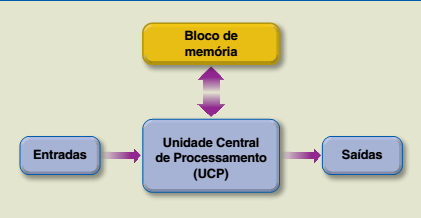
\includegraphics[width=.9\textwidth, keepaspectratio]{../figs/cap04/constituicao.png}
				\end{figure}
		
			\end{column}
		\end{columns}
	\end{frame}
	
	\begin{frame}{Unidade Central de Processamento}
		\begin{itemize}
			\item Responsável pelas operações lógicas e aritméticas
			\vspace{1em}
			\item Controla e supervisiona toda a operação do CLP
			\vspace{1em}
			\item Velocidade de operação definida pela frequência de \textit{clock}
		\end{itemize}
	\end{frame}	
	
	\begin{frame}{Blocos de memória}
		\begin{itemize}
			\item Armazena os programas e dados de operação do sistema
			\vspace{1em}
			\item Arquitetura Harvard
			\begin{itemize}
				\item Memória de programas e dados \alert{separadas}
			\end{itemize}
		\end{itemize}
		
	\end{frame}
	
	\begin{frame}{Entradas/Saídas digitais}
		\begin{columns}
			\begin{column}{0.5\textwidth}
				\begin{itemize}
					\item Entradas
					\begin{itemize}
						\item Chaves \textit{push button}
						\item Chaves fim de curso
						\item Contatos de relés
						\item Sensores de proximidade 
						\item Sensores de presença
						\item Termostatos
						\item Pressostatos
					\end{itemize}
					
				\end{itemize}
			\end{column}
			\begin{column}{0.5\textwidth}
				\begin{itemize}
					\item Saídas
					\begin{itemize}
						\item Lâmpadas
						\item Relés de controle
						\item Buzinas
						\item Válvulas elétricas 
						\item Solenóides
						\item Disjuntores
						\item Motores
					\end{itemize}
					
				\end{itemize}
			\end{column}
		\end{columns}
	\end{frame}
	
	\begin{frame}{Outros componentes}
		\begin{itemize}
			\item Fonte de alimentação
			\vspace{1em}
			\item Terminal de programação
			\vspace{1em}
			\item Bloco de comunicações
			\vspace{1em}
			\item Interface Homem Máquina

		\end{itemize}
	\end{frame}
	
	\begin{frame}{Funcionalidades}
				\begin{figure}[hbtp]
				\centering
				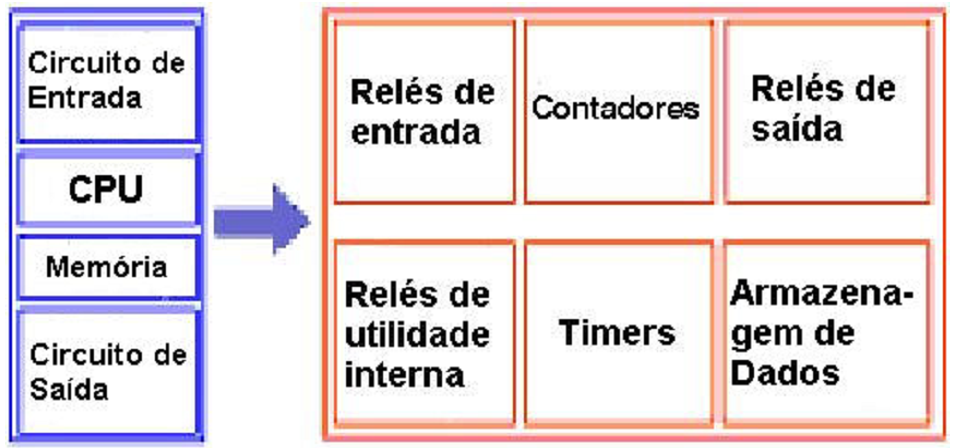
\includegraphics[height=5cm, keepaspectratio]{../figs/cap04/funcionalidades.png}
				\end{figure}
	\end{frame}
	
	\begin{frame}[allowframebreaks]{Funcionalidades}
		
		\begin{itemize}
			\item Relés de entrada
			\begin{itemize}
				\item Conectados com o mundo externo
			\end{itemize}
			\vspace{1em}
			\item Relés de utilidade interna
			\begin{itemize}
				\item Não recebem sinais do mundo
				\item Relés simulados
			\end{itemize}
			\vspace{1em}
			\item Relés de sáida
			\framebreak
			\item Contadores
			\begin{itemize}
				\item Contagem de pulsos
				\item Crescente ou decrescente
			\end{itemize}
			\vspace{1em}
			\item Temporizadores
			\begin{itemize}
				\item Funções de retardo
			\end{itemize}
		\end{itemize}
	\end{frame}

	\begin{frame}{Classificação dos CLPs}
		\begin{eftable}
			\begin{tabular}{c||c}
			\textcolor{white}{PORTE} & \textcolor{white}{NÚMERO DE PONTOS} \\ 
			Micro & $\pm$ 20 \\ 
			Mini & $\pm$ 180 \\ 
			Pequeno & $\pm$ 400 \\
			Médio & Até 3000 \\ 
			Grande & Acima de 3000 \\ 
			\end{tabular} 
		
		\end{eftable}
	\end{frame}

	\begin{frame}{Estrutura de Programação}
	
	\begin{columns}
			\begin{column}{0.5\textwidth}
				\begin{figure}[hbtp]
				\centering
				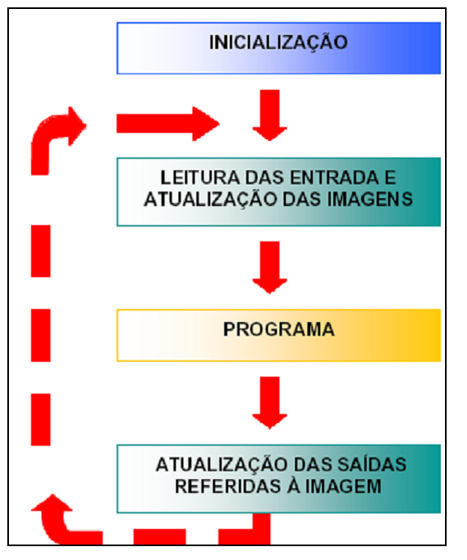
\includegraphics[height=5cm, keepaspectratio]{../figs/cap04/fluxograma.png}
				\end{figure}
			\end{column}
			\begin{column}{0.5\textwidth}
				\begin{figure}[hbtp]
				\centering
				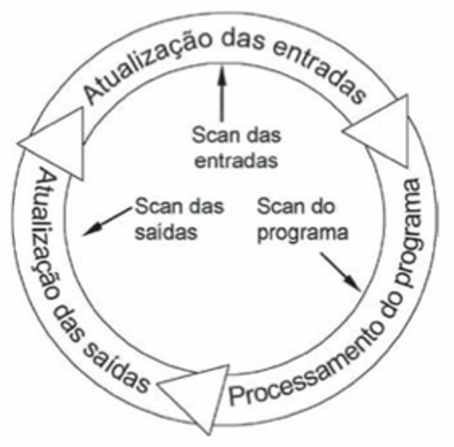
\includegraphics[height=5cm, keepaspectratio]{../figs/cap04/scan.png}
				\end{figure}
			\end{column}
		\end{columns}	
	\end{frame}

	\begin{frame}[allowframebreaks]{Aspectos de software}
		\begin{itemize}
			\item Linguagens de Programação - IEC 61131-3
			\begin{itemize}
				\item Ladder
				\item Texto Estruturado (ST - \textit{Structured Text})
				\item Lista de Instruções (IL - \textit{Instruction List})
				\item Diagrama de blocos funcionais (FBD - \textit{Function Block Diagram})
			\end{itemize}
			\vspace{1em}
			\framebreak
			\item Operações permitidas
			\begin{itemize}
				\item Aritmética básica ($+$, $-$, $*$)
				\item Lógica AND, OR, XOR
				\item Temporização e contagem
				\item Comparação de valores
				\item Ponto flutuante
				\item Leitura de sinais analógicos
				\item Malha de controle PID
				\item Lógica Fuzzy				
			\end{itemize}
		\end{itemize}
	\end{frame}

	\begin{frame}{Escolha de um CLP}
		\begin{itemize}
			\item Número de entradas
			\vspace{1em}
			\item Número de saídas
			\vspace{1em}
			\item Velocidade de processamento
			\vspace{1em}
			\item Tipos de entrada e saída
			\vspace{2.5em}
			
			\begin{center}
				\centering
				\Huge
				\alert{Olhar especificações do CLP}
			\end{center}
		\end{itemize}
	\end{frame}
	
	\begin{frame}{}
	\end{frame}
	
\end{document}
